\documentclass[10pt, 
]{IEEEtran}
\usepackage{graphicx}
\usepackage{amsmath}
\usepackage{hyperref}
\usepackage{listings}
\usepackage{xcolor}
\usepackage{booktabs} 
 
\title{RepliCode: Deterministic Execution for WebAssembly}

\author{
    \IEEEauthorblockN{Ricardo Perelló Mas}
    \IEEEauthorblockA{
        EPFL \\
        ricardo.perellomas@epfl.ch
    }
}

\begin{document}

\maketitle

\begin{abstract}
RepliCode introduces a deterministic WebAssembly runtime that ensures consistent execution across distributed systems. By leveraging a NAT-inspired network layer and deterministic I/O operations, RepliCode addresses the challenges of non-deterministic behavior in replicated environments. This report details the system's design, implementation, and evaluation, highlighting its contributions to deterministic execution and elastic scaling.
\end{abstract}

\section{Introduction}
RepliCode tackles the problem of deterministic execution in distributed systems, where traditional approaches suffer from non-deterministic I/O and limited scalability. Our system introduces a deterministic runtime with elastic scaling capabilities, achieved through a NAT layer that ensures consistent operation ordering. This report outlines our contributions, including a deterministic I/O abstraction, NAT-inspired network management, and a runtime synchronization mechanism.

\section{Contributions}
\subsection{Deterministic Network Operation Layer}
\begin{itemize}
    \item Introduces a novel approach for deterministic network operations across runtime instances.
    \item Utilizes a NAT layer for consistent operation order and timing.
    \item Key innovations include port mapping, connection management, and buffering mechanisms.
\end{itemize}

\subsection{Process Isolation and Port Management}
\begin{itemize}
    \item Provides a method for process isolation within replicated environments.
    \item Assigns isolated port spaces managed by the NAT layer.
    \item Ensures deterministic port assignment across instances.
\end{itemize}

\subsection{Runtime Synchronization Mechanism}
\begin{itemize}
    \item Proposes a mechanism for dynamic and deterministic runtime synchronization.
    \item Enables new instances to join and sync with global state without halting execution.
\end{itemize}

\section{System Design}

The RepliCode architecture consists of two core components: a centralized \textbf{consensus server} and multiple distributed \textbf{replicated runtimes}. The consensus server coordinates external I/O operations and enforces deterministic execution by maintaining and broadcasting ordered sequences of operations known as \emph{batches}. Critically, \textbf{all communication} between the consensus server and runtimes occurs exclusively through these batches, ensuring strict determinism and consistency across the system.

A \textbf{batch} is an ordered set of high-level \emph{commands}, representing either user inputs or external system events. Each batch is finalized by appending a logical clock tick, creating a global timeline shared by all runtimes. Batches are generated at fixed intervals controlled by a timer within the consensus server. Although this interval is configurable via recompilation, batches cannot be triggered manually, thus ensuring deterministic progression across the system.

\subsection{Consensus Server}

The consensus server acts as the central authority and performs four primary roles:

\begin{itemize}
\item \textbf{NAT Module:} Provides deterministic network management, handling port mappings, message routing, and maintaining network state consistency.
\item \textbf{Runtime Manager:} Manages runtime connections, session states, and runtime availability. If a runtime disconnects, it is immediately removed from the distribution list to maintain consistency.
\item \textbf{HTTP Server:} Publishes NAT mappings publicly, allowing external clients to discover the correct ports for interacting with services running inside runtimes.
\item \textbf{Command Interface:} Accepts user commands via a command-line interface (CLI), buffering them until the batch timer triggers batch creation.
\end{itemize}

Upon each timer expiration, the consensus server aggregates buffered user commands and intercepted I/O operations, appends a logical timestamp, and broadcasts this batch to all connected runtimes. All batches are persistently logged.

\subsection{Runtime Design}

Each runtime is sandboxed and executes batches deterministically. Runtimes consist of the following key components:

\begin{itemize}
\item \textbf{Consensus Input Buffer:} Stores incoming batches from the consensus server until they are ready for processing.
\item \textbf{Deterministic Scheduler:} Controls execution of processes according to batch order and local runtime state, ensuring deterministic outcomes.
\item \textbf{I/O Interceptor:} Captures all system calls related to external operations, redirecting them through consensus-managed pathways.
\item \textbf{Outgoing Buffer:} Collects intercepted I/O calls, bundling them into an outgoing batch sent back to the consensus server before processing new incoming batches.
\end{itemize}

Each runtime maintains detailed per-process metadata—including execution state, blocking conditions, and a local NAT table—to facilitate deterministic scheduling decisions. Importantly, each process maintains its own isolated NAT state, distinct from the public NAT mappings maintained by the consensus server.

Since runtimes deterministically execute identical incoming batches, their outgoing batches are inherently identical. To optimize network usage, the consensus server accepts the first received outgoing batch from any runtime, discarding duplicates.

The RepliCode architecture abstracts network interactions completely. Both clients and internal processes perceive their interactions as direct socket communication, while all underlying coordination—such as batching and NAT mappings—is hidden, preserving conventional networking semantics.

\subsection{Synchronization Mechanism}
When a new runtime instance joins the system, it must be brought into a fully consistent state with respect to existing replicas. RepliCode achieves this through a dedicated synchronization mechanism implemented by the consensus server’s runtime manager.

Upon connection, the runtime manager assigns the new runtime a unique identifier and retrieves all previously issued incoming batches from the persistent batch log. These batches represent the entire historical sequence of system events. The manager sequentially transmits these batches to the new runtime in the exact order they were originally generated. Because all commands are deterministic and batches encode a complete history, the joining runtime reconstructs its state precisely from the initial execution state to the present.

Critically, determinism at the runtime level is guaranteed by stripping inherent non-determinism from external I/O at the consensus level, which ensures that all instructions are uniformly ordered within batches. Subsequently, each runtime, using re-implemented deterministic system calls and a custom scheduler, ensures that identical inputs and state produce exactly the same result. This combined approach results in total state determinism, allowing runtimes to synchronize seamlessly and remain consistently synchronized thereafter.

This mechanism guarantees that newly connected runtimes behave identically to existing ones and can participate in future batch processing immediately after synchronization—without disrupting consensus or requiring any global pause. This elasticity is a cornerstone of RepliCode’s design, enabling dynamic scaling and fault recovery with minimal operational overhead.

\subsection{Execution Flow}

The following steps illustrate the high-level execution flow in RepliCode:

\begin{enumerate}
\item The consensus server initializes and begins accepting runtime connections.
\item New runtimes connect and are synchronized by receiving and replaying all historical incoming batches.
\item Runtimes execute commands in the precise order dictated by incoming batches.
\item When a runtime process issues an external I/O call, it is intercepted and buffered.
\item Buffered I/O calls are sent back as an outgoing batch to the consensus server before the next incoming batch is processed.
\item The consensus server processes these outgoing batches, updating NAT state, and prepares any resulting events (e.g., network responses) for inclusion in the subsequent batch.
\item Updated batches are sent to runtimes, continuing the deterministic execution loop.
\end{enumerate}


\subsection{NAT Layer Operation}

The NAT module provides deterministic management of network interactions. It operates through a structured mapping mechanism, maintaining consistent port assignments and connection states across all runtimes. The key components and responsibilities of the NAT module include:

\begin{itemize}
\item \textbf{Port Allocation and Mapping:} The NAT assigns public ports deterministically to internal process ports upon request, maintaining consistent mappings across all replicas. Each process-port pair receives a unique public port to avoid conflicts.
\item \textbf{Connection Management:} NAT tracks connections initiated by runtimes, maintaining mappings between internal and consensus-level ports. It manages connection lifecycles explicitly, handling establishment, data forwarding, and termination deterministically.
\item \textbf{Buffering and Forwarding:} Incoming data from external clients is buffered by NAT until requested by processes. NAT forwards data deterministically, ensuring all runtimes receive identical data streams at the same points in their execution.
\item \textbf{Non-blocking Operations and Waiting States:} Operations such as \texttt{accept} and \texttt{recv} may temporarily block if no data or connections are available. NAT manages these states explicitly, marking operations as waiting and resuming them once the relevant events occur.
\end{itemize}

This deterministic and structured approach ensures consistent network behavior across all runtime replicas, facilitating strong consistency.


\subsection{NAT Interaction Example}

The following example demonstrates deterministic NAT interactions, where an image server is running inside a runtime with process id = 2 and an external client is sending requests to the server, with diagrams illustrating the step-by-step communication:

\textbf{Step 1 (Connection Setup):}
\begin{enumerate}
\item Server process listens on internal port 7000.
\item Consensus server assigns public port 10000 mapped to \texttt{pid2:7000}.
\item Server blocks waiting for client connection.
\item Client queries consensus HTTP server, discovering public port 10000 for \texttt{pid2:7000}.
\item Client initiates connection to port 10000.
\item Consensus registers new connection, assigning internal port 8000 and public port 10001.
\item Connection setup completes successfully.
\end{enumerate}

\begin{figure}[h]
\centering
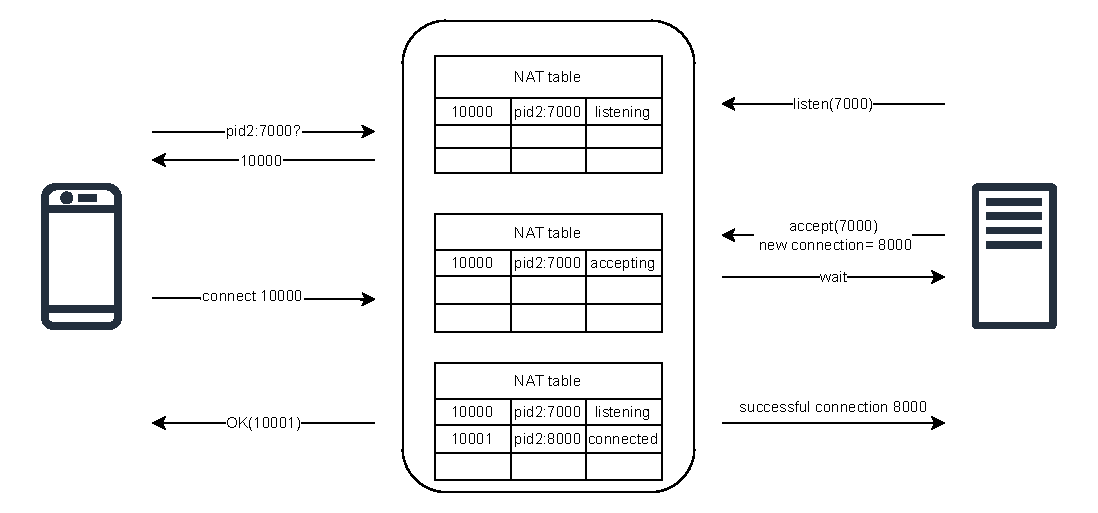
\includegraphics[width=0.9\linewidth]{consensus_diagram_1.pdf}
\caption{Step 1: Initial connection setup and port assignment.}
\label{fig:consensus-1}
\end{figure}

\textbf{Step 2 (Data Transfer):}
\begin{enumerate}
\item Client sends file \texttt{lake.jpg} to port 10001.
\item Server reads data from internal port 8000.
\item NAT forwards data deterministically.
\item Server closes the connection, and NAT cleans up mappings.
\end{enumerate}

\begin{figure}[h]
\centering
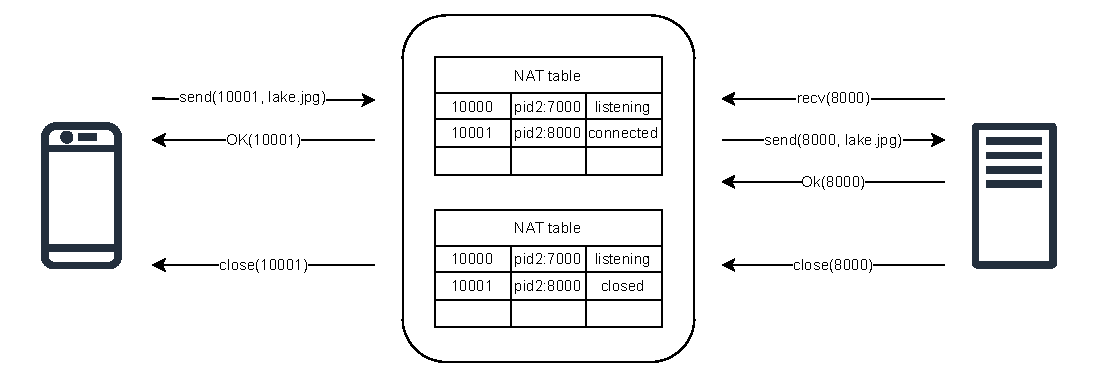
\includegraphics[width=0.9\linewidth]{consensus_diagram_2.pdf}
\caption{Step 2: Deterministic message routing and data transfer.}
\label{fig:consensus-2}
\end{figure}

\textbf{Step 3 (Handling Additional Connections):}
\begin{enumerate}
\item Server accepts new connection on internal listener port 7000.
\item Client connects via public port 10000.
\item NAT assigns new public port 10002.
\item Client sends request \texttt{"GET lake.jpg"} to port 10002.
\item NAT forwards request to internal port 8001.
\item Server responds, and NAT forwards the response back to the client.
\item Connection closes gracefully.
\end{enumerate}

\begin{figure}[h]
\centering
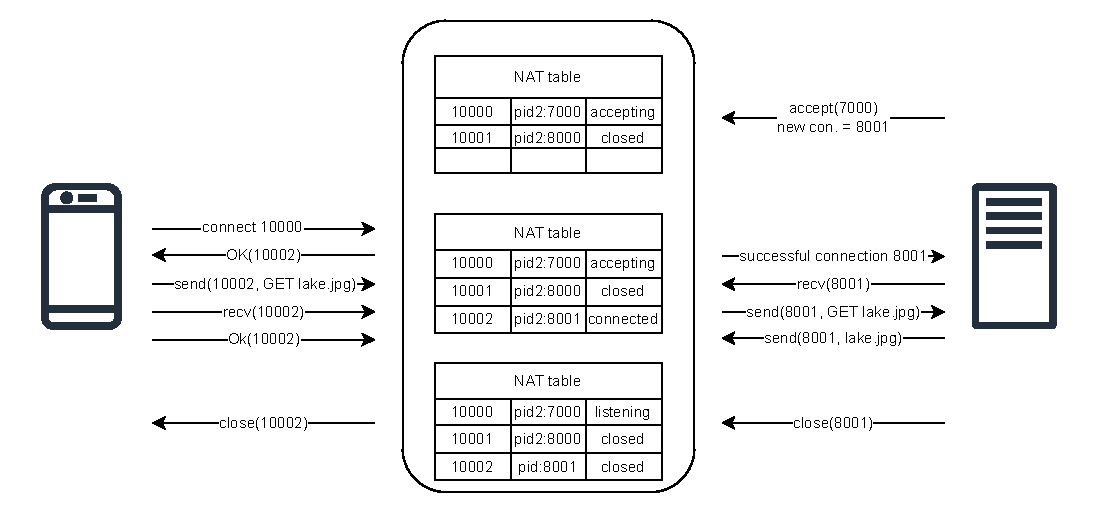
\includegraphics[width=0.9\linewidth]{consensus_diagram_3.pdf}
\caption{Step 3: Handling new connections and request/response flow.}
\label{fig:consensus-3}
\end{figure}

Figures \ref{fig:consensus-1}, \ref{fig:consensus-2}, and \ref{fig:consensus-3} visually represent each step of this deterministic interaction.


\section{Implementation Details}

This section describes specific design choices and internal mechanics that support the deterministic execution model in RepliCode.

\subsection{Batch Structure}

\begin{verbatim}
struct Batch {
    number: u64,
    direction: BatchDirection,
    data: Vec<u8>,
}  
\end{verbatim}



Batches are either \texttt{Incoming} (from consensus to runtime) or \texttt{Outgoing} (from runtime to consensus). A runtime sends its outgoing batch prior to receiving a new incoming one.

\subsection{Command Internals}

\begin{verbatim}
enum Command {
    Clock(u64),
    Init { wasm\_bytes, dir\_path, args },
    FDMsg(pid, Vec<u8>),
    NetworkIn(pid, port, data),
    NetworkOut(pid, NetworkOperation),
}
\end{verbatim}


\subsection{Network Operations}

Networking is modeled through a NAT module, and operations such as \texttt{Connect}, \texttt{Accept}, \texttt{Send}, and \texttt{Recv} are encoded as \texttt{NetworkOperation} variants. These are intercepted and batched by the runtime, then routed through consensus to ensure determinism.

\subsection{Blocking and Scheduler Unblocking}

Processes may become blocked due to I/O operations. For example, a process calling \texttt{accept()} is marked \texttt{Blocked(NetworkIO)}. Upon receiving a \texttt{NetworkIn} message in the next batch, the runtime checks if the process can now resume. This decision is made by inspecting the process’s own metadata, which includes a local NAT table and socket state.

\begin{quote}
\textbf{A process remains blocked if \emph{any} of the following hold:}
\begin{itemize}
\item It is waiting on an \texttt{accept()} call and no incoming connection has arrived.
\item It is waiting to \texttt{recv()} data and the socket buffer is empty.
\item It is a listening socket that hasn't yet been assigned a consensus-level port.
\end{itemize}
\end{quote}

If none of these conditions hold, the scheduler:
\begin{itemize}
\item Marks the process as \texttt{Ready}.
\item Clears the blocking reason.
\item Signals the process to resume execution.
\end{itemize}

\subsection{Runtime Batch Processing}

The runtime processes consensus input in the following order:
\begin{enumerate}
\item Sends any outgoing network messages first.
\item Reads the incoming batch header, length, and data.
\item Parses the data into records (e.g., \texttt{Init}, \texttt{FDMsg}, \texttt{NetworkIn}, etc.).
\item Updates runtime state accordingly (e.g., modifying NAT tables, writing buffers, or spawning processes).
\end{enumerate}

An example \texttt{NetworkIn} handler inspects whether a success status was received (e.g., for \texttt{accept()}), and if so, updates the NAT table and connected flag for the relevant socket. If not, it may retain the block or mark the operation as failed. The process is then notified using a condition variable.

This layer acts as the bridge between consensus-level message propagation and per-runtime state evolution.

\section{Evaluation}

\subsection{Setup}
\textbf{Hardware:} All experiments were conducted on one machine with an M4 PRO CPU, 48 GB of RAM, and SSD storage, connected via a WiFi. \\ 
\textbf{Software:} The consensus server and each runtime were compiled using Rust (debug profile) and executed on macOS. File transfers were performed using a TCP-based image server--NAT--client interface.

\subsection{Experiment 1: Network Overhead}
\textbf{Question:} What is the overhead introduced by the deterministic NAT layer in terms of bytes, throughput, and latency? \\ 
\textbf{Method:} We compared file transfers between a direct client-server setup and one using the NAT layer. Transfers used 4 KB batching. \\ 
\textbf{Results:}
\newline

\begin{tabular}{|l|l|l|l|}
\hline
\textbf{File} & \textbf{Size} & \textbf{NAT Bytes} & \textbf{Overhead (\%)} \\ \hline
small-image.jpg & 3.6 KB & 3642 & 0.75\% \\ \hline
big-image.jpg & ~2.0 MB & 2101449 & 0.17\% \\ \hline
\end{tabular} \\ 
\newline
\textbf{Observations:} Overhead remained constant (27 bytes) per batch. Relative overhead dropped as file size increased. Throughput was unaffected. \\ 
\textbf{Deductions:} Larger batch sizes reduce the relative cost of NAT metadata. The NAT layer provides determinism with negligible performance impact. \\ 
\textbf{Conclusion:} The NAT layer introduces minimal and predictable overhead.

\subsection{Experiment 2: Consistent File Transfers}
\textbf{Question:} Does the NAT layer ensure consistent operation ordering and data delivery across all runtime instances? \\ 
\textbf{Method:} Three runtime servers were launched. Clients performed SEND and GET operations for various file sizes via the NAT. \\ 
\textbf{Observations:} All runtime logs showed identical command sequences. File contents and chunking were identical. Timestamps were synchronized. \\ 
\textbf{Deductions:} The NAT layer enforces a consistent global operation order. \\ 
\textbf{Conclusion:} The system guarantees strong consistency and deterministic behavior across replicas.

\subsection{Experiment 3: Concurrent Operations}
\textbf{Question:} Can the NAT layer maintain deterministic behavior when multiple clients perform overlapping operations? \\ 
\textbf{Method:} Two clients initiated conflicting SEND and GET operations. \\ 
\textbf{Observations:} The NAT layer serialized requests by connection order. Logs were identical. \\ 
\textbf{Deductions:} The NAT's queue-based design prevents races. \\ 
\textbf{Conclusion:} First-come, first-served behavior guarantees consistent replay.

\subsection{Experiment 4: Buffer Management and Delivery Consistency}
\textbf{Question:} How well does the NAT layer’s buffering maintain delivery consistency under stress? \\ 
\textbf{Method:} We varied send intervals during large file transfers. \\ 
\textbf{Observations:} Receiving path robust at \( < 1\,\text{ms} \) intervals. Sending path corrupted messages below 15ms. \\ 
\textbf{Deductions:} Reliable delivery requires send intervals \( \geq 15 \)ms. \\ 
\textbf{Conclusion:} System is deterministic but sensitive to batching frequency.

\subsection{Experiment 5: Deterministic Port Assignment}
\textbf{Question:} Does the system assign ports deterministically across replicas without conflicts? \\ 
\textbf{Method:} We launched two WASM services (image and key-value servers). \\ 
\textbf{Observations:} Port assignment was disjoint, deterministic, and consistent across replicas. \\ 
\textbf{Deductions:} Determinism is achieved via local monotonic counters. \\ 
\textbf{Conclusion:} Port assignment is deterministic, conflict-free, and isolated by design.

\subsection{Experiment 6: Dynamic Scaling}
\textbf{Question:} How efficiently can new runtime instances synchronize with the system during execution? \\ 
\textbf{Method:} We launched runtimes A, B, and C at staggered intervals and recorded synchronization metrics. \\ 
\textbf{Results:} Latency remained below 211 ms with linear metadata cost. No consensus disruption. \\ 
\textbf{Conclusion:} Elastic scaling is feasible with minimal delay.

\subsection{Experiment 7: State Consistency During Operation}
\textbf{Question:} Do mid-execution joins preserve system consistency during I/O activity? \\ 
\textbf{Method:} Live file uploads continued as new runtimes joined. \\ 
\textbf{Observations:} Logs and file states remained identical. No data loss. \\ 
\textbf{Conclusion:} Synchronization mechanism preserves strong consistency during ongoing operations.

\subsection{Summary}
The evaluation confirms that our deterministic NAT layer and synchronization mechanisms provide minimal overhead, preserve strong consistency, and support elastic scaling. Concurrent access and high-throughput stress are handled robustly. These properties validate our design for deterministic, replicated runtime environments.
\section{Related Work}
RepliCode builds on deterministic RSMs, deterministic I/O, and elastic cloud computing, extending these concepts to WebAssembly in distributed systems.

\section{Conclusion}
RepliCode addresses the challenges of deterministic execution in distributed systems, providing a robust and scalable solution. Future work includes support for multi-threading and larger-scale deployments.

\bibliographystyle{IEEEtran}
\bibliography{references}

\end{document}